В графическом интерфейсе необходимо было предусмотреть выбор директорий для работы системы и вывод информации.

Для создания интерфейса использовался Qt Designer --- кроссплатформенная свободная среда для разработки графических интерфейсов (GUI, англ. <<Graphic User Interface>>) программ, использующих библиотеку Qt. Входит в состав Qt framework. При разработке использовался механизм слотов. Сигналы и слоты --- подход, который позволяет реализовать шаблон <<наблюдатель>>, минимизируя написание повторяющегося кода. Концепция заключается в том, что компонент может посылать сигналы, содержащие информацию о событии. В свою очередь другие компоненты могут принимать эти сигналы посредством специальных функций --- слотов. Данный механизм является основной идеей в QT и подходит для описания графического интерфейса пользователя.

Так как система <<COEX>> является консольной утилитой, то графический интерфейс генерирует строку с необходимыми параметрами и запускает с ними консольную утилиту, перехватывая вывод и отображая его в интерфейсе. В качестве параметров выступают директории для работы системы. Главное окно представлено на рисунке~\ref{ship_1:ship_1}.

\begin{figure}[h!]
\center{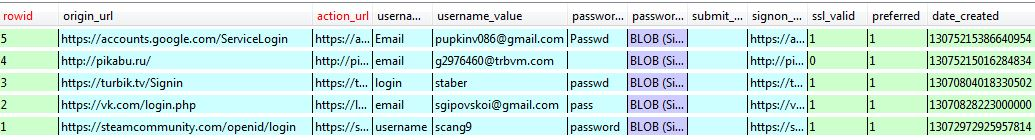
\includegraphics[width=0.5\linewidth]{ship_1}}
\caption{ Главное окно интерфейса }
\label{ship_1:ship_1}
\end{figure}

Интерфейс состоит из следующих элементов:
\begin{enumerate}
  \item кнопка <<Открыть папку>> --- отвечает за выбор папки, в которой будет производиться поиск;
  \item кнопка <<Сохранить в папку>> --- отвечает за выбор папки для сохранения результатов; 
  \item в данном окне отображается вывод процесса выполнения;
  \item кнопка <<Запуск>> --- отвечает за запуск системы;
  \item окно, в котором находятся текущие плагины для выполнения в виде списка. 
\end{enumerate}

Если не были выбраны директории для работы, то при нажатии на кнопку <<Запуск>> отобразится соответствующее сообщение (рис.~\ref{ship_2:ship_2}). Диалоговое окно выбора директории представлено на рисунке~\ref{ship_3:ship_3}. Процесс выполнения программы представлен на рисунке~\ref{ship_4:ship_4}. По завершении работы системы отобразится соответствующие сообщение (рис.~\ref{ship_5:ship_5}).

\begin{figure}[h!]
\center{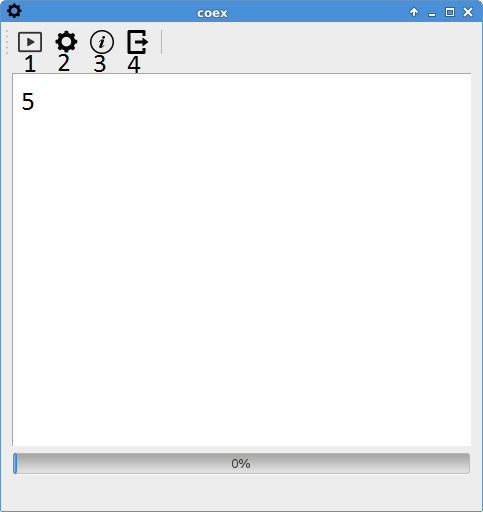
\includegraphics[width=0.5\linewidth]{ship_2}}
\caption{ Сообщение об ошибке }
\label{ship_2:ship_2}
\end{figure}

\begin{figure}[h!]
\center{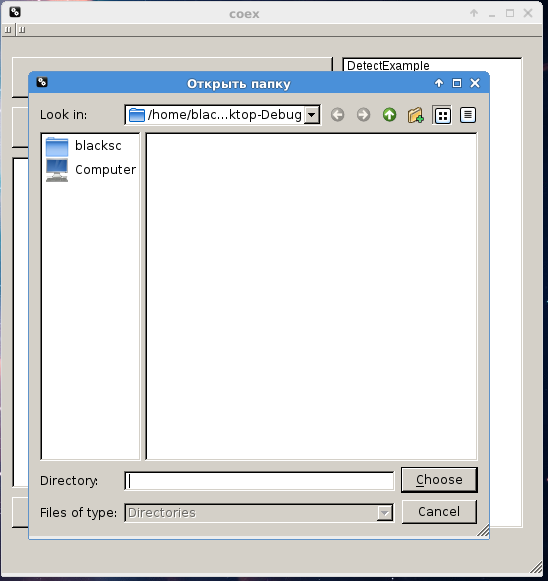
\includegraphics[width=0.5\linewidth]{ship_3}}
\caption{ Выбор директории }
\label{ship_3:ship_3}
\end{figure}

\begin{figure}[h!]
\center{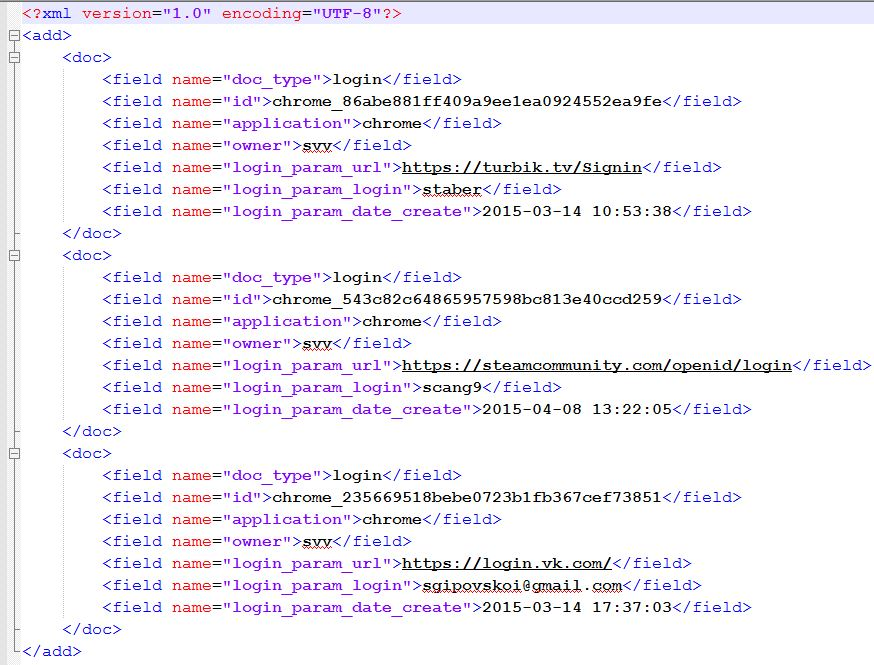
\includegraphics[width=0.5\linewidth]{ship_4}}
\caption{ Процесс выполнения программы }
\label{ship_4:ship_4}
\end{figure}

\begin{figure}[h!]
\center{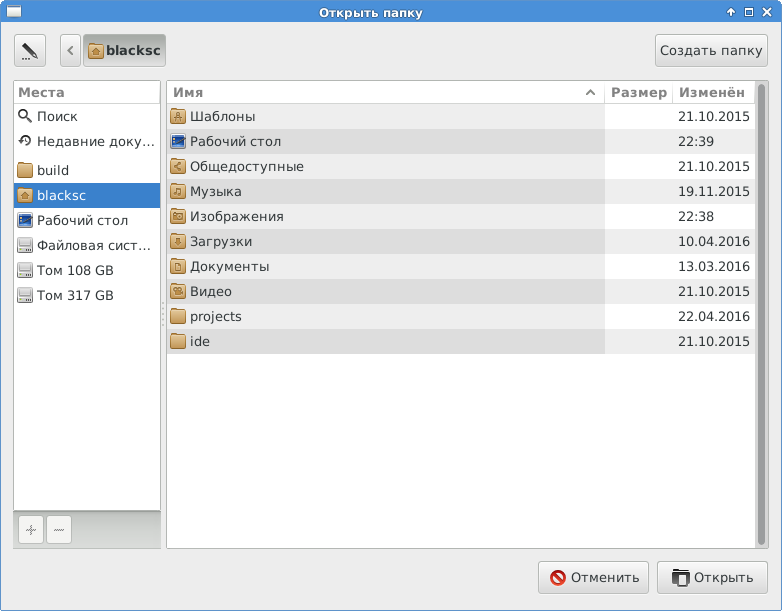
\includegraphics[width=0.5\linewidth]{ship_5}}
\caption{ Сообщение о выполнении }
\label{ship_5:ship_5}
\end{figure}







